\chapter{Implementacja}
\label{cha:implementacja}

Agent mając wiedzę na temat
\begin{itemize*}
\renewcommand{\labelitemi}{$\bullet$}
 \item akcji, które może wykonać,
 \item stanu, w jakim się znajduje,
 \item zasad, definiujących warunki otrzymania nagrody,
 \item polityki wybierania akcji
\end{itemize*}
jest w stanie dostosować swoje kolejne działania (wybrane akcje), tak aby uzyskać jak
najlepszy wynik w kolejnych iteracjach symulacji. Celem agenta jest dotarcie do punktu końcowego, zdobywając jak 
największą nagrodę. \\
\indent Po osiągnięciu celu symulacja jest resetowana, jej wynik jest zapisywany. Robot ucząc się na podstawie 
poprzednio dokonanych wyborów, buduje tablicę mapującą stan-akcja $Q(S, A)$ do konkretnej wyliczonej wartości. W 
programie do przedstawienia wartości tablicy stan-akcja $Q(S, A)$ wykorzystano wielowymiarową tablicę.

\section{Tablica stan-akcja $Q(S, A)$}

Tablica $Q(S, A)$ jest to struktura danych przechowująca wszystkie stany i możliwe do wykonania w nich akcje. Każdej z tych akcji przyporządkowana jest odpowiednia wartość, która jest poddawana modyfikacji przez odpowiedni algorytm uczenia ze wzmocnieniem.
Ostatecznym celem działania algorytmu jest uzyskanie takich informacji w strukturze $Q(S, A)$, aby robot korzystając z polityki optymalnej (tzn. takiej, w której agent wybiera zawsze najlepszą według niego akcję) wykonał cel z jak najlepszym wynikiem.

W programie zaimplementowana jest funkcja drukowania wyników symulacji do arkusza kalkulacyjnego, przykładowy wpis 
zaprezentowany jest na rys. \ref{fig:przykladowywpis}.


\begin{figure}[H]
    \centering
    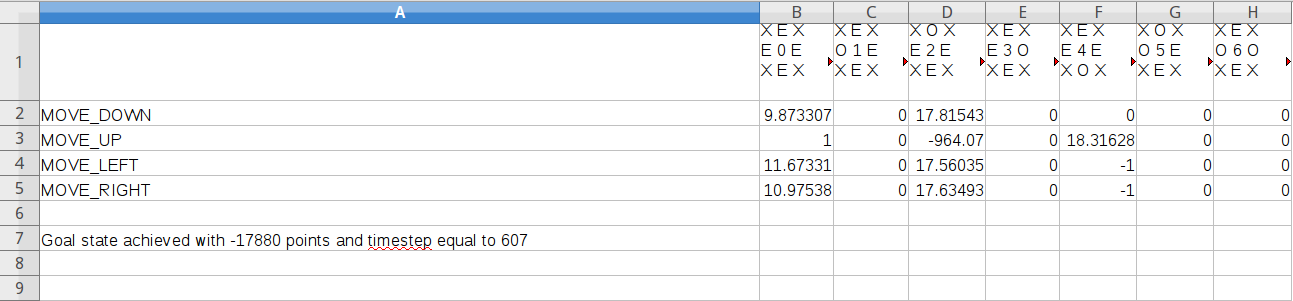
\includegraphics[scale=0.4]{przykladowywpis}
    \caption{Przykładowy wynik działania algorytmu Q-learning. Można zauważyć, że do każdego stanu przydzielone są 
akcję wraz z wartością skumulowanej nagrody wyliczonej za pomocą algorytmu.}
    \label{fig:przykladowywpis}
\end{figure}

Na rys. \ref{fig:wyjasnieniewpisu} przedstawiono znaczenie symboli w pojedynczym wpisie.

\begin{figure}[H]
    \centering
    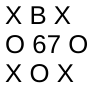
\includegraphics[scale=1]{wyjasnieniewpisu}
    \caption{Liczba w samym środku reprezentuje numer stanu. Bezpośrednią z nią sąsiadujące są typy obiektów, 
\textbf{B}order - granica, \textbf{O}stacle - przeszkoda, \textbf{E}mpty - puste pole, \textbf{P}rize - nagroda (stan 
końcowy)
    \label{fig:wyjasnieniewpisu}
\end{figure}


\section{Polityka wyboru akcji}
\label{sec:politykawyboru}

Agent mając do dyspozycji jedną z możliwych akcji $a$ ze zbioru wszystkich akcji $A$, musi podjąć decyzje, która akcję 
ma wybrać jako następną. W tej implementacji rozważane są dwie polityki
\begin{enumerate}
	\item $\epsilon$-greedy policy
	\item optimal policy
\end{enumerate}

\subsection{Równowaga pomiędzy eksploracją, a eksploatacją}
Od wyboru polityki zależy stopień eksploracji algorytmu. Gdyby agent za każdym razem wybierał najbardziej korzystną według niego akcję, byłby podatny na zakleszczenie w nieoptymalnym rozwiązaniu. Wprowadzając pewną losowość wyboru akcji agent, będzie w stanie odkryć nowe rozwiązania, nawet jeżeli według jego aktualnej wiedzy znalazł to najbardziej optymalne. Powstało dużo prac dokładniej badających to zagadnienie \ref{thrun1992efficient}, \ref{wiewiora2004efficient}.

\subsection{$\epsilon$-greedy policy}

Polityka $\epsilon$-greedy jest strategią wyboru akcji polegającą na wyborze losowej akcji z prawdopodobieństwem $\epsilon$, a w przeciwnym wypadku wybranie najbardziej korzystnej. Agent wybiera akcję, która według niego będzie najbardziej korzystna z prawdopodobieństwem $1-\epsilon$, a w przeciwnym wypadku wykonuje akcję losową. Parametr $\epsilon$ jest regulowany zależnie od potrzeb i musi spełniać zależność $0 < \epsilon < 1$.

\subsection{Optimal policy}

Polityka optymalna, agent za każdym razem wybiera najkorzystniejszą według jego wiedzy akcję.

\section{Symulacja graficzna}
\label{sec:symulacjagraficzna}

Jako symulację graficzna działania algorytmu wykorzystano figury geometryczne reprezentujące: agenta, przeszkody, 
granice i cel.
Agent porusza się na dwuwymiarowej przestrzeni o wymiarach $50*50$ pikseli.

Przykładowy stan środowiska w symulacji przedstawiono na rys. \ref{fig:symulacja}, \ref{fig:symulacja2}.

\begin{figure}[H]
    \centering
    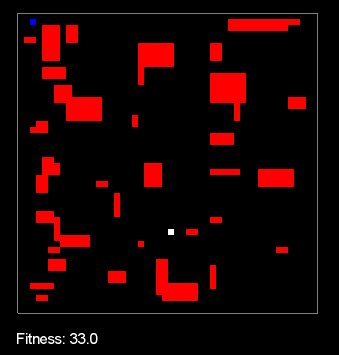
\includegraphics[scale=0.6]{symulacja}
    \caption{Przykładowy stan symulacji}
    \label{fig:symulacja}
\end{figure}

\begin{figure}[H]
    \centering
    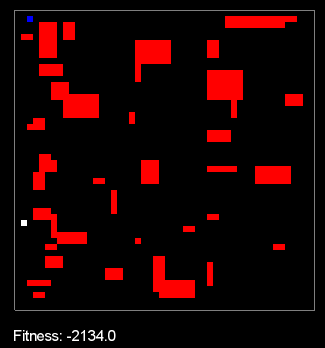
\includegraphics[scale=0.6]{symulacja2}
    \caption{Przykładowy stan symulacji}
    \label{fig:symulacja2}
\end{figure}

Na rys. \ref{fig:symulacja}, \ref{fig:symulacja2}, można zauważyć następującą reprezentacje obiektów jako kolor:
\begin{itemize}
\renewcommand{\labelitemi}{$\bullet$}
 \item czerwony - przeszkoda,
 \item biały - agent,
 \item niebieski - nagroda,
 \item szary - granica.
\end{itemize}


\section{Reprezentacja stanu}
\label{sec:reprezentacjastanu}

Stan w jakim znajduje się aktualnie robot jest przedstawiony w postaci siatki $3*3$. Agent jest świadomy obiektów 
znajdujących się nad nim, pod nim oraz po jego prawej i lewej stronie.
Agent może napotkać następujące obiekty
\begin{description}
%\renewcommand{\labelitemi}{$\bullet$}
 \item przeszkoda $(O)$, robot \textbf{może} wejść na przeszkodę, jednak traci za to określoną liczbę punktów;
 \item nagroda $(P)$, stan końcowy. Gdy agent osiąga cel symulacja zapisuje wynik działania i uruchamia się kolejny 
epizod nauki robota;
 \item granica $(B)$, granica jest obiektem wyznaczającym pole symulacji, dlatego też nie jest możliwe przemieszczenie 
się na nią;
  \item puste pole $(E)$, pole nie zawierające żadnego z pozostałych obiektów;
\end{description}
 
Przykładowe stany w jakich może się znaleźć robot przedstawiono na rys. \ref{fig:grid1}, \ref{fig:grid2}, 
\ref{fig:grid3} i \ref{fig:grid4}.

\begin{figure}[H]
    \centering
    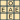
\includegraphics[scale=10]{grid1}
    \caption{Agent graniczy od górnej strony z przeszkodą, natomiast w pozostałych kierunkach znajdują się puste pola}
    \label{fig:grid1}
\end{figure}

\begin{figure}[H]
    \centering
    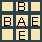
\includegraphics[scale=10]{grid2}
    \caption{Agent graniczy od góry i lewej strony z granicą, oznacza to, że robot znajduje się w górnym lewym rogu 
mapy, a jedynymi akcjami jakie może wykonać to ruch w prawo i ruch w dół}
    \label{fig:grid2}
\end{figure}

\begin{figure}[H]
    \centering
    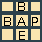
\includegraphics[scale=10]{grid3}
    \caption{Agent graniczy od góry i lewej strony z granicą, a od prawej z stanem końcowym. Agent wykonując 
ruch w prawo osiągnie swój cel, powodując tym samym zakończenie i zresetowanie symulacji}
    \label{fig:grid3}
\end{figure}

\begin{figure}[H]
    \centering
    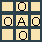
\includegraphics[scale=10]{grid4}
    \caption{Agent graniczy z każdej strony z przeszkodą, jakikolwiek ruch powoduje utratę punktów}
    \label{fig:grid4}
\end{figure}

\subsection{Akcje}
\label{subsec:akcje}

Robot znajdując się w dowolnym stanie nie graniczącym z obiektem $B$ (granicą), jest w stanie wykonać jedną z czterech 
akcji:

\begin{enumerate}
 \item ruch do góry,
 \item ruch do dołu,
 \item ruch w prawo,
 \item ruch w lewo.
\end{enumerate}

Agent \textbf{nie może} przemieścić się na granicę, w związku z czym w przypadku sąsiedztwa z granicą, robot posiada 
ograniczony zakres ruchów. 

\subsection{Wartość nagród}

Algorytm, aby wiedzieć czy akcja, którą wykonał jest korzystna czy nie musi otrzymywać nagrodę. W zaimplementowanym 
środowisku robot dostaje ujemną nagrodę o wartości(-1) po wykonaniu jakiegokolwiek ruchu na puste pole. Dzięki temu 
zabiegowi agent stara się jak najszybciej dojść do celu, wykonując jak najmniejszą liczbę ruchów. Aby utrudnić 
dojście do celu agentowi, wprowadzono ujemną nagrodę o wartości -200 po kontakcie z przeszkodą. Robot dąży do 
odnalezienia takiej drogi, która nie przebiega przez przeszkody. Za dojście do celu uzyskuje pozytywny sygnał o wartości 
1000.

Początkowo takie rozwiązanie wydawało się działać prawidłowo, jednak miało jedną poważną wadę. Agent bardzo długi czas 
spędzał w początkowych etapach symulacji, nie wiedząc w która stronę powinien się udać, aby dojść do celu. Dlatego 
wprowadzono pozytywną nagrodę o wartości 2, za każdy ruch w stronę nagrody.

\subsection{Wybór algorytmów}
\label{subsec:wyboralgorytmow}

Do implementacji inteligentnego zachowania agenta, wybrano algorytm Q-learning z dziedziny uczenia ze wzmocnieniem.
Wartość parametrów:
\begin{itemize}
 \item discount factor: 0.7
 \item learning rate: 0.6
 \item $\epsilon$: 0.2
\end{itemize}

Na listingu \ref{lst:qlearning} przedstawiono implementację algorytmu Q-learning.

\lstset{language=Java,
	basicstyle=\ttfamily,
	keywordstyle=\color{blue}\ttfamily,
	stringstyle=\color{red}\ttfamily,
	commentstyle=\color{gray}\ttfamily,
	morecomment=[l][\color{magenta}]{\#}
	frame=single, % adds a frame around the code
	tabsize=2, % sets default tabsize to 2 spaces
	breaklines=true, % sets automatic line breaking
}
\begin{lstlisting}[caption=Implementacja algorytmu Q-learning, label={lst:qlearning}, captionpos=b, 
belowcaptionskip=4pt]

        State currentState, nextState;
        Action currentAction;

//        lowers discount factor after an arbitrary amount of time
        if(renderTimer % 1000 == 0 && discountFactor > 0){
            System.out.println("lowering discountFactor");
            discountFactor -= 0.1d;
        }

        if(renderTimer % threshold == 0){

//            start out in an initial state as the current state
            currentState = State.identifyState(agent.getX(), agent.getY(), 
Environment.getInstance().getEnvironmentState());
            List<Action> currentlyPossibleActions = new ArrayList<>(qValues.get(currentState).keySet());

//            select one among all possible actions for the current state
//            epsilon-greedy policy takes random action once in a while, otherwise chooses the best one
            double d = Math.random();
            if (d > epsilon){

//                get best action for current state
                double Qmax = qValues.get(currentState).get(currentlyPossibleActions.get(0));
                Action bestAction = null;

                for(Map.Entry<Action, Float> actionEntry : qValues.get(currentState).entrySet()){
                    if(actionEntry.getValue() >= Qmax){
                        Qmax = actionEntry.getValue();
                        bestAction = actionEntry.getKey();
                    }
                }
                if(bestAction == null){
                    for(Map.Entry<Action, Float> actionEntry : qValues.get(currentState).entrySet())
                        System.out.println(actionEntry);
                    throw new NullPointerException("Empty action!");
                }
                currentAction = bestAction;
            }
            else {
//                random action
                currentAction = currentlyPossibleActions.get(ThreadLocalRandom.current().nextInt(0, 
currentlyPossibleActions.size()));
            }

//            consider transitioning to state, after executing current action
            nextState = State.considerNextState(currentAction, agent.getX(), agent.getY());

//            find qMax for nextState
            float Qmax = 0;

            for(Map.Entry<Action, Float> actionEntry : qValues.get(nextState).entrySet()){
                if(actionEntry.getValue() > Qmax){
                    Qmax = actionEntry.getValue();
                }
            }

//            get the reward for the (current state, current action, next state) tuple
            float reward = agent.returnReward(currentState, currentAction, agent.getX(), agent.getY());


//            update Q value
            float currentStateQValue = qValues.get(currentState).get(currentAction);
            float qValue = currentStateQValue + learningRate *(reward + discountFactor *Qmax - currentStateQValue);
            qValues.get(currentState).put(currentAction, qValue);


//            set current state to next state
            currentState = nextState;

            agent.move(currentAction, Gdx.graphics.getDeltaTime());
            timeStep++;

            return reward;
\end{lstlisting}

\section{Wykorzystane technologie}
\label{sec:wykorzystanetechnologie}

Java 8 kod został napisany w języku Java. Do generowania grafiki została wykorzystana biblioteka LibGDX. W celu notowania wyników do plików kalkulacyjnych została wykorzystana biblioteka Apache POI.
W celu zmniejszenia ilości kodu użyto biblioteki Project Lombok, pozwalającej na automatyczne generowane getterów, 
setterów, konstruktorów lub metod hashcode i equals. Do budowania i zarządzania projektem wykorzystano narzędzie Gradle.

\section{Napotkane problemy}
\label{sec:napotkaneproblemy}

Przy projektowaniu aplikacji, największy problem stanowiło odpowiednie przedstawienie aktualnego stanu środowiska i robota. Nieodpowiednie odwzorowanie stanu, może powodować niepoprawną naukę agenta.
Zakładając rozmiar mapy $50*50$, można zauważyć, że przy naiwnej reprezentacji stanu, tzn. takiej, w której każda możliwa kombinacja stanu mapy jest reprezentowana osobno, powstaje ogromna ilość możliwych akcji w tablicy wartości $Q(S,A)$ 
Ostatecznie postanowiono przedstawić stan w postaci siatki $3*3$.

Kolejnym problemem, który napotkano przy implementacji działania algorytmów jest ich testowanie. Algorytmy uczenia ze 
wzmocnieniem są niełatwymi metodami do testowania, niepoprawność działania agenta może wynikać z wielu różnych błędów 
implementacji, jak również z niepoprawnego modelu środowiska czy reprezentacji stanu. Negatywnie na 
działanie robota wpływają też nieodpowiednio dobrane parametry implementacji lub polityki.

\section{Obsługa symulacji}

Do obsługi symulacji zostały zaimplementowane następujące funkcje:
\begin{itemize}
 \item Spowolnienie symulacji - wciskając przycisk $-$, można spowolnić działanie symulacji
 \item Przyspieszenie symulacji - wciskając przycisk $+$, można przyspieszyć działanie symulacji
 \item Zresetowanie symulacji - klawisz $ENTER$ służy do resetowania symulacji
 \item Zmiana polityki robota - używając przycisku $p$, można sterować polityką robota wybierając pomiędzy 
$\epsilon$-greedy, a optimal policy
\end{itemize}


\section{Wynik działania}
\label{sec:wynikdzialania}

Algorytm z łatwością poradził sobie z wyznaczeniem najkrótszej, najbardziej korzystnej drogi w 
zaprojektowanym środowisku. Po niedługim procesie nauki, robot generuje skuteczną tablice wartości $Q(S, A)$.
Jako, że zaimplementowany został algorytm off-policy Q-learning, można zaobserwować brak wpływu nauczania na politykę 
wybierania akcji. Pomimo to, że agent znalazł już satysfakcjonujące rozwiązanie to nadal jest zaangażowany w eksploracje 
nowych stanów. Gdyby wykorzystano algorytm on-policy SARSA, robot pod wpływem uzyskanych wyników zmienił by strategię 
wyboru kolejnych akcji, wykorzystując politykę optymalną. Przykładowe wyniki przedstawiono na rys. \ref{fig:wynik1}, 
\ref{fig:wynik2} i \ref{fig:wynik3}.

\begin{figure}[H]
    \centering
    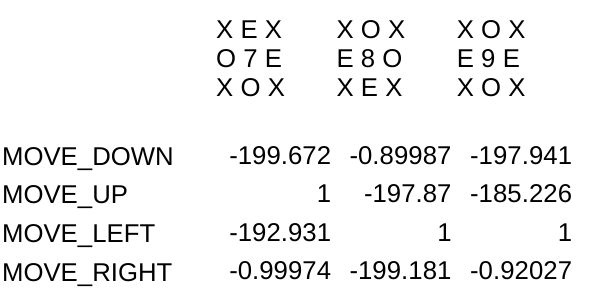
\includegraphics[scale=0.7]{wynik1}
    \caption{Przykładowy wynik działania algorytmu. Można zaobserwować poprawnie wyznaczone wartości akcji. Nagroda 
znajduje się w lewym górnym rogu mapy, dlatego też nie opłaca się agentowi wykonać akcję w przeciwnym kierunku. Agent 
jeżeli ma taką możliwość wykonuje ruch w takich stan, żeby nie znaleźć się na przeszkodzie}
    \label{fig:wynik1}
\end{figure}

\begin{figure}[H]
    \centering
    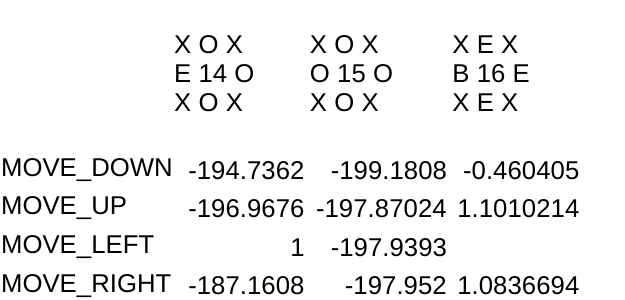
\includegraphics[scale=0.7]{wynik2}
    \caption{Przykładowy wynik działania algorytmu. Podobnie jak na obrazku wyżej, agent wykonuje podobne wybory. Można 
zauważyć, że agent znajdując się wewnątrz przeszkody (stan nr. 15), każdy ruch uważa za niekorzystny ale jednak z 
delikatną przewagą do góry lub w lewo (w kierunku nagrody). W przypadku, gdy agent graniczy z lewej strony z przeszkodą 
jak w stanie nr. 16, niedostępna jest akcja MOVE LEFT}
    \label{fig:wynik2}
\end{figure}

\begin{figure}[H]
    \centering
    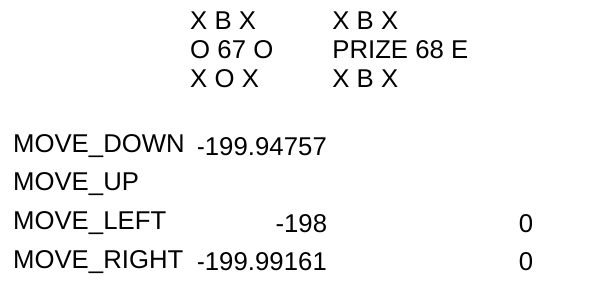
\includegraphics[scale=0.7]{wynik3}
    \caption{Przykładowy wynik działania algorytmu. Na tym obrazku widać stan nr. 68, w którym agent nigdy się nie 
znalazł. Jest to logiczna konsekwencja tego, że nagroda (stan końcowy) znajduje się w lewym górnym obszarze mapy, a 
więc nie może sąsiadować z granicą od dołu}
    \label{fig:wynik3}
\end{figure}



%---------------------------------------------------------------------------














